\documentclass[zavrsnirad]{fer}
% Dodaj opciju upload za generiranje konačne verzije koja se učitava na FERWeb
% Add the option upload to generate the final version which is uploaded to FERWeb


\usepackage{blindtext}



%--- PODACI O RADU / THESIS INFORMATION ----------------------------------------

% Naslov na engleskom jeziku / Title in English
\title{Machine Learning Model for Alzheimer's Disease Classification Using Brain MRI Images}

% Naslov na hrvatskom jeziku / Title in Croatian
\naslov{Model strojnog učenja za klasifikaciju Alzheimerove bolesti uporabom slika magnetske rezonancije mozga}

% Broj rada / Thesis number
\brojrada{1291}

% Autor / Author
\author{Petra Buršić}

% Mentor 
\mentor{Doc.dr.sc\@ Jelena Božek}

% Datum rada na engleskom jeziku / Date in English
\date{June, 2024}

% Datum rada na hrvatskom jeziku / Date in Croatian
\datum{lipanj, 2024.}

%-------------------------------------------------------------------------------


\begin{document}


% Naslovnica se automatski generira / Titlepage is automatically generated
\maketitle


%--- ZADATAK / THESIS ASSIGNMENT -----------------------------------------------

% Zadatak se ubacuje iz vanjske datoteke / Thesis assignment is included from external file
% Upiši ime PDF datoteke preuzete s FERWeb-a / Enter the filename of the PDF downloaded from FERWeb
\zadatak{zadatak.pdf}


%--- ZAHVALE / ACKNOWLEDGMENT --------------------------------------------------

\begin{zahvale}
  % Ovdje upišite zahvale / Write in the acknowledgment
  Hvala na kavi...
\end{zahvale}


% Odovud započinje numeriranje stranica / Page numbering starts from here
\mainmatter


% Sadržaj se automatski generira / Table of contents is automatically generated
\tableofcontents


%--- UVOD / INTRODUCTION -------------------------------------------------------
\chapter{Uvod}
\label{pog:uvod}

Alzheimerova bolest (AD) predstavlja jedan od najvećih medicinskih i društvenih izazova suvremenog doba. Prema podacima Svjetske zdravstvene organizacije, AD je vodeći uzrok demencije, stanja koje trenutno pogađa preko 50 milijuna ljudi širom svijeta, a predviđa se da će se taj broj udvostručiti svakih 20 godina, dosežući 152 milijuna do 2050. godine \cite{PMID:29763097}. U Hrvatskoj, gdje oko 16\% populacije čine osobe starije od 65 godina, procjenjuje se da oko 80,000 ljudi pati od demencije, od čega većinu čine pacijenti s Alzheimerovom bolesti \cite{MIMICA2010409}. Ova bolest karakterizira progresivni gubitak kognitivnih funkcija, što značajno narušava svakodnevni život pojedinca i njegovih skrbnika. Rana dijagnoza AD-a može značajno pomoći u upravljanju simptomima i planiranju skrbi, ali trenutno ne postoji pouzdani lijek koji bolest može izliječiti ili znatno usporiti njezin napredak \cite{PMID:29763097}.
\\
Demencija, kao rezultat AD-a, uzrokuje značajne promjene u mozgu. Jedna od glavnih karakteristika je nakupljanje beta-amiloidnih plakova izvan neurona i neurofibrilarnih čvorova unutar neurona.\cite{10.1007/s00500-020-05292-x} Oni dovode do smrti moždanih stanica i gubitka sinaptičke veze između neurona. Kao posljedica toga, dolazi do atrofije mozga, posebno u područjima koja su ključna za pamćenje, kao što je hipokampus, te u korteksu koji je odgovoran za mišljenje, planiranje i pamćenje \cite{doi:10.1212/WNL.0b013e3181c3f293}.
\\
MRI, posebno strukturni MRI, je neinvazivna tehnika snimanja koja pruža detaljne slike anatomije mozga. Široko se koristi za otkrivanje strukturnih promjena u mozgu povezanih s AD-om, kao što su atrofija hipokampusa i promjene u kortikalnoj debljini \cite{10.3389/fnins.2015.00307}. 
\\
Strojno učenje pruža moćne alate za analizu velikih skupova podataka i može značajno unaprijediti sposobnost dijagnoze složenih bolesti poput AD-a. Algoritmi strojnog učenja mogu analizirati obrasce u MRI slikama i prepoznati suptilne promjene koje možda nisu odmah vidljive stručnjacima, čime se povećava točnost i učinkovitost dijagnoze.
\\
Uz pomoć strukturnih MRI slika iz baze podataka Alzheimer’s Disease Neuroimaging Initiative (ADNI), u ovom radu primijenit ćemo dvije metode strojnog učenja, Decision Tree (DT) i Support Vector Machine (SVM), kako bismo razvili, testirali i usporedili modele sposobne za klasifikaciju pojedinaca u tri kategorije: zdrave osobe (CN), osobe s blagim kognitivnim oštećenjem (MCI) i osobe s Alzheimerovom bolešću (AD).


%-------------------------------------------------------------------------------
\chapter{Glavni dio}
\label{pog:glavni_dio}

\section{Magnetna rezonanca (MRI)}

Magnetna rezonanca (MRI) je neinvazivna tehnika snimanja koja koristi magnetska polja i radiovalove za stvaranje detaljnih slika unutarnjih struktura tijela. Konvencionalna MRI se široko koristi za radiološku dijagnozu i stvara prostorne mape svojstava mobilnih vodikovih jezgri (protona) koje se uglavnom nalaze u molekulama vode. Kontrast unutar slika proizlazi iz varijacija u gustoći vode unutar tkiva i načinu na koji voda reagira s makromolekulama \cite{Gore2003}. Postoje tri glavne vrste MRI-a: strukturni MRI (sMRI), funkcionalni MRI (fMRI) i difuzijski MRI (dMRI).


\subsection{Strukturni MRI (sMRI)}
Strukturni MRI (sMRI) je ključan za diferencijalnu dijagnozu Alzheimerove bolesti (AD) zbog svoje sposobnosti vizualizacije specifičnih obrazaca atrofije u mozgu. Najčešće patološke značajke povezane s demencijom su kortikalna atrofija, uključujući atrofiju medijalnog temporalnog režnja, i vaskularne promjene. U AD-u se često primjećuje kontinuirani gubitak neurona, posebno u medijalnom temporalnom režnju (MTL), gdje atrofija prvo zahvaća entorinalno područje, a zatim hipokampus, amigdalu i parahipokampus \cite{Promteangtrong2015}. U ovom radu koristimo strukturne MRI slike iz ADNI baze podataka kako bismo razvili, testirali i usporedili modele strojnog učenja za klasifikaciju Alzheimerove bolesti. Korištenje strukturnih MRI podataka omogućuje precizno identificiranje regija mozga koje su zahvaćene AD-om, što je ključno za razumijevanje progresije bolesti i razvoj učinkovitih metoda za njezinu dijagnozu i praćenje \cite{Gonuguntla2022}.


\subsection{Funkcionalni MRI (fMRI)}

Funkcionalni MRI (fMRI) koristi se za detekciju malih promjena u signalima koji se koriste za proizvodnju magnetsko-rezonantnih slika koje su povezane s neuronskom aktivnošću u mozgu. fMRI detektira promjene ovisne o razini kisika u krvi (BOLD) koje se javljaju kada se promjene u neuronskoj aktivnosti dogode nakon promjene stanja mozga, poput stimulusa ili zadatka. Ova tehnika je sigurna, neinvazivna i ponovljiva kod odraslih i djece, te ima široke potencijalne primjene u osnovnoj i kliničkoj neuroznanosti (Gore, 2003) \cite{Gore2003}. Na slici \ref{fig:fMRI_BOLD} prikazana je promjena BOLD (Blood-Oxygen-Level Dependent) signala u odnosu na neuronsku aktivnost, ilustrirajući kako fMRI detektira metaboličke promjene povezane s neuronskom aktivnošću.

\begin{figure}[h]
	\centering
	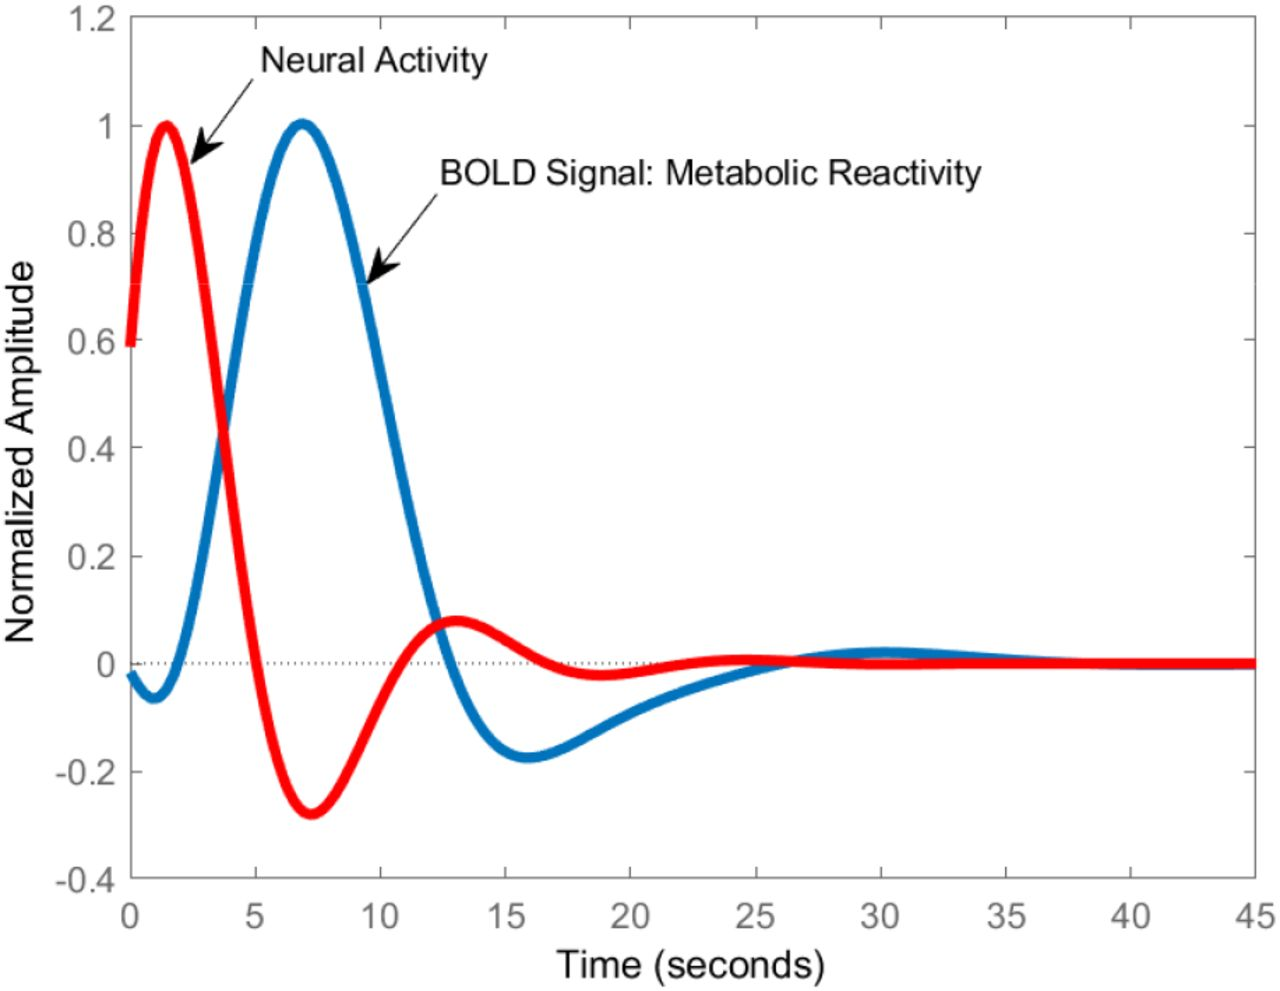
\includegraphics[width=0.6\textwidth]{Figures/BOLD.jpg}
	\caption{Promjena BOLD (Blood-Oxygen-Level Dependent) signala u odnosu na neuronsku aktivnost.\cite{Schaper573006}}
	\label{fig:fMRI_BOLD}
\end{figure}


\subsection{Difuzijski MRI (dMRI)}
Difuzijski MRI (dMRI) koristi se za mjerenje difuzije molekula vode u tkivima, što može pružiti informacije o mikrostrukturi mozga. dMRI tehnika može otkriti mikroskopske promjene u tkivima u ranim fazama AD-a, poput gubitka mijelina, oštećenja aksona i gubitka neurona. Ove promjene mogu biti ključne za rano otkrivanje i praćenje progresije bolesti \cite{Promteangtrong2015}.


\subsection{Primjena MRI-a u istraživanju AD-a}

\section{Podaci i metode}
\subsection{ADNI baza podataka}
\subsection{Prikupljanje i predobrada MRI slika}
\subsection{Značajke izdvojene iz MRI slika}

\section{Modeli strojnog učenja}
\subsection{Decision Tree (DT)}
\subsubsection{Teorijska osnova}
\subsubsection{Implementacija}
\subsection{Support Vector Machine (SVM)}
\subsubsection{Teorijska osnova}
\subsubsection{Implementacija}

\section{Trening i validacija modela}
\subsection{Podjela podataka}
\subsection{Evaluacijske metrike (točnost, osjetljivost, specifičnost)}





%-------------------------------------------------------------------------------
\chapter{Rezultati i rasprava}
\label{pog:rezultati_i_rasprava}

\subsection{Rezultati}
\subsubsection{Performanse DT modela}
% Vaš tekst ovdje

\subsubsection{Performanse SVM modela}
% Vaš tekst ovdje

\subsubsection{Usporedba modela}
% Vaš tekst ovdje

\subsubsection{Vizualizacija rezultata}
% Vaš tekst ovdje

\subsection{Rasprava}
\subsubsection{Analiza rezultata}
% Vaš tekst ovdje

\subsubsection{Prednosti i ograničenja korištenih modela}
% Vaš tekst ovdje

\subsubsection{Usporedba s postojećim studijama}
% Vaš tekst ovdje

\subsubsection{Potencijalne implikacije za kliničku praksu}
% Vaš tekst ovdje


%--- ZAKLJUČAK / CONCLUSION ----------------------------------------------------
\chapter{Zaključak}
\label{pog:zakljucak}



%--- LITERATURA / REFERENCES ---------------------------------------------------

% Literatura se automatski generira iz zadane .bib datoteke / References are automatically generated from the supplied .bib file
% Upiši ime BibTeX datoteke bez .bib nastavka / Enter the name of the BibTeX file without .bib extension
\bibliography{literatura}



%--- SAŽETAK / ABSTRACT --------------------------------------------------------

% Sažetak na hrvatskom
\begin{sazetak}
  Unesite sažetak na hrvatskom.


\end{sazetak}

\begin{kljucnerijeci}
  prva ključna riječ; druga ključna riječ; treća ključna riječ
\end{kljucnerijeci}


% Abstract in English
\begin{abstract}
  Enter the abstract in English.
  
  \blindtext 
\end{abstract}

\begin{keywords}
  the first keyword; the second keyword; the third keyword
\end{keywords}


%--- PRIVITCI / APPENDIX -------------------------------------------------------

% Sva poglavlja koja slijede će biti označena slovom i riječi privitak / All following chapters will be denoted with an appendix and a letter
\backmatter

\chapter{The Code}




\end{document}
